\documentclass[sigplan]{acmart}

\usepackage[T1]{fontenc}
\usepackage{lmodern}
\usepackage[utf8]{inputenc}

%% Some recommended packages.
\usepackage{booktabs}   %% For formal tables:
                        %% http://ctan.org/pkg/booktabs
\usepackage{subcaption} %% For complex figures with subfigures/subcaptions
% DOI
\acmDOI{10.475/123_4}

% ISBN
\acmISBN{123-4567-24-567/08/06}

%Conference
\acmConference[IWST'17]{International Workshop on Smalltalk Technologies}{ESUG 2017}{Maribor, Slovenia 4-8 September 2017} 
%\acmYear{1997}
\copyrightyear{2017}

%\acmPrice{15.00}

%\acmBadgeL[http://ctuning.org/ae/ppopp2016.html]{ae-logo}
%\acmBadgeR[http://ctuning.org/ae/ppopp2016.html]{ae-logo}



\usepackage[T1]{fontenc} %%%key to get copy and paste for the code!
\usepackage[utf8]{inputenc} %%% to support copy and paste with accents for frnehc stuff
%\usepackage{times}
%\usepackage[scaled=0.85]{helvet}
\usepackage{graphicx}
\usepackage{ifthen}
\usepackage{xspace}
\usepackage{alltt}
\usepackage{latexsym}
\usepackage{url}            
\usepackage{amssymb}
\usepackage{amsfonts}
\usepackage{amsmath}
\usepackage{stmaryrd}
\usepackage{enumerate}
%\usepackage{cite}
% \usepackage[pdftex,colorlinks=true,pdfstartview=FitV,linkcolor=blue,citecolor=blue,urlcolor=blue]{hyperref}
%\usepackage{xspace}
%\newcommand*{\eg}{e.g.\@\xspace}
%\newcommand*{\ie}{i.e.\@\xspace}

\makeatletter
\newcommand*{\etc}{%
    \@ifnextchar{.}%
        {etc}%
        {etc.\@\xspace}%
}
\makeatother

\usepackage{float}
% \usepackage{xcolor}
% \usepackage{listings}
% \usepackage{highlight}

%\usepackage{multicol}
\usepackage{url}
\usepackage{multicol}

% \usepackage
% [
%   left=20mm,
%   right=20mm,
%   top=30mm,
%   bottom=30mm,
%   bindingoffset=10mm
%   % use vmargin=2cm to make vertical margins equal to 2cm.
%   % use hmargin=3cm to make horizontal margins equal to 3cm.
%   % use margin=3cm to make all margins  equal to 3cm.
% ] {geometry}

\newboolean{showcomments}
\setboolean{showcomments}{true}
\ifthenelse{\boolean{showcomments}}
  {\newcommand{\bnote}[2]{
	\fbox{\bfseries\sffamily\scriptsize#1}
    {\sf\small$\blacktriangleright$\textit{#2}$\blacktriangleleft$}
    % \marginpar{\fbox{\bfseries\sffamily#1}}
   }
   \newcommand{\cvsversion}{\emph{\scriptsize$-$Id: macros.tex,v 1.1.1.1 2007/02/28 13:43:36 bergel Exp $-$}}
  }
  {\newcommand{\bnote}[2]{}
   \newcommand{\cvsversion}{}
  } 


\newcommand{\here}{\bnote{***}{CONTINUE HERE}}
\newcommand{\nb}[1]{\bnote{NB}{#1}}

\newcommand{\fix}[1]{\bnote{FIX}{#1}}
%%%% add your own macros 

\newcommand{\ab}[1]{\bnote{Alex}{#1}}
\newcommand{\sd}[1]{\bnote{Stef}{#1}}
\newcommand{\ja}[1]{\bnote{Jannik}{#1}}
\newcommand{\md}[1]{\bnote{MD}{#1}}
\newcommand{\jr}[1]{\bnote{JRe}{#1}}
\newcommand{\lf}[1]{\bnote{Luc}{#1}}

\graphicspath{{figures/}}
%%% 


\newcommand{\figref}[1]{Figure~\ref{fig:#1}}
\newcommand{\figlabel}[1]{\label{fig:#1}}
\newcommand{\tabref}[1]{Table~\ref{tab:#1}}
\newcommand{\layout}[1]{#1}
\newcommand{\commented}[1]{}
\newcommand{\secref}[1]{Section \ref{sec:#1}}
\newcommand{\seclabel}[1]{\label{sec:#1}}

%\newcommand{\ct}[1]{\textsf{#1}}
\newcommand{\stCode}[1]{\textsf{#1}}
\newcommand{\stMethod}[1]{\textsf{#1}}
\newcommand{\sep}{\texttt{>>}\xspace}
\newcommand{\stAssoc}{\texttt{->}\xspace}

\newcommand{\stBar}{$\mid$}
\newcommand{\stSelector}{$\gg$}
\newcommand{\ret}{\^{}}
\newcommand{\msup}{$>$}
%\newcommand{\ret}{$\uparrow$\xspace}

\newcommand{\myparagraph}[1]{\noindent\textbf{#1.}}
\newcommand{\eg}{\emph{e.g.,}\xspace}
\newcommand{\ie}{\emph{i.e.,}\xspace}
\newcommand{\etal}{\emph{et al.,}\xspace}
\newcommand{\ct}[1]{{\textsf{#1}}\xspace}


\newenvironment{code}
    {\begin{alltt}\sffamily}
    {\end{alltt}\normalsize}

\newcommand{\defaultScale}{0.55}
\newcommand{\pic}[3]{
   \begin{figure}[h]
   \begin{center}
   \includegraphics[scale=\defaultScale]{#1}
   \caption{#2}
   \label{#3}
   \end{center}
   \end{figure}
}

\newcommand{\twocolumnpic}[3]{
   \begin{figure*}[!ht]
   \begin{center}
   \includegraphics[scale=\defaultScale]{#1}
   \caption{#2}
   \label{#3}
   \end{center}
   \end{figure*}}

\newcommand{\infe}{$<$}
\newcommand{\supe}{$\rightarrow$\xspace}
\newcommand{\di}{$\gg$\xspace}
\newcommand{\adhoc}{\textit{ad-hoc}\xspace}

\usepackage{url}            
\makeatletter
\def\url@leostyle{%
  \@ifundefined{selectfont}{\def\UrlFont{\sf}}{\def\UrlFont{\small\sffamily}}}
\makeatother
% Now actually use the newly defined style.
\urlstyle{leo}



%\setlength\parindent{0pt}

% \date{}

% Just add % Just add % Just add \input{smalltalkEnv} to your file
% then you can use :
% \begin{lstlisting}[language=Smalltalk]
% false become: true.
% \end{lstlisting}

\usepackage{color}
\usepackage{listings}
\usepackage{etoolbox}

\definecolor{stComment}{rgb}{0.5,0.5,0.5}
\definecolor{stString}{rgb}{0.58,0,0.82}
\definecolor{stKeywords}{rgb}{0.21,0.55,0.7}
\definecolor{stNumbers}{rgb}{.5,0,0}

\newtoggle{InString}{}% Keep track of if we are within a string
\togglefalse{InString}% Assume not initally in string
\newcommand*{\ColorIfNotInString}[1]{\iftoggle{InString}{#1}{\color{stNumbers}#1}}%
\newcommand*{\ProcessQuote}[1]{#1\iftoggle{InString}{\global\togglefalse{InString}}{\global\toggletrue{InString}}}%

\lstdefinelanguage{Smalltalk}{
  keywordstyle=\color{stKeywords},
  commentstyle=\color{stComment},
  stringstyle=\color{stString},
  alsoletter=\#,
  identifierstyle=\idstyle, 
  showstringspaces=false,
  morekeywords={true,false,self,super,nil},
  sensitive=true, 
  morecomment=[s]{"}{"}, 
  morestring=[d]', 
  style=SmalltalkStyle,
  tabsize=2,
}


\makeatletter%
\newcommand*\idstyle[1]{%
  \expandafter\id@style\the\lst@token{#1}\relax%
}
\def\id@style#1#2\relax{%
  \ifnum\pdfstrcmp{#1}{\#}=0%
  \ttfamily\color{stString} \the\lst@token%
  \else%
  \edef\tempa{\uccode`#1}%
  \edef\tempb{`#1}%
  \ifnum\tempa=\tempb%
  \ttfamily\color{blue} \the\lst@token%
  \else%
  \the\lst@token%
  \fi%
  \fi%
}

\lstdefinestyle{SmalltalkStyle}{ 
  literate=%
  {^}{{$\uparrow$}}1% 
  % {"}{{{\ProcessQuote{"}}}}1% Disable coloring within double quotes
  % {'}{{{\ProcessQuote{'}}}}1% Disable coloring within single quote
  {0}{{{\ColorIfNotInString{0}}}}1%
  {1}{{{\ColorIfNotInString{1}}}}1%
  {2}{{{\ColorIfNotInString{2}}}}1%
  {3}{{{\ColorIfNotInString{3}}}}1%
  {4}{{{\ColorIfNotInString{4}}}}1%
  {5}{{{\ColorIfNotInString{5}}}}1%
  {6}{{{\ColorIfNotInString{6}}}}1%
  {7}{{{\ColorIfNotInString{7}}}}1%
  {8}{{{\ColorIfNotInString{8}}}}1%
  {9}{{{\ColorIfNotInString{9}}}}1%
}  to your file
% then you can use :
% \begin{lstlisting}[language=Smalltalk]
% false become: true.
% \end{lstlisting}

\usepackage{color}
\usepackage{listings}
\usepackage{etoolbox}

\definecolor{stComment}{rgb}{0.5,0.5,0.5}
\definecolor{stString}{rgb}{0.58,0,0.82}
\definecolor{stKeywords}{rgb}{0.21,0.55,0.7}
\definecolor{stNumbers}{rgb}{.5,0,0}

\newtoggle{InString}{}% Keep track of if we are within a string
\togglefalse{InString}% Assume not initally in string
\newcommand*{\ColorIfNotInString}[1]{\iftoggle{InString}{#1}{\color{stNumbers}#1}}%
\newcommand*{\ProcessQuote}[1]{#1\iftoggle{InString}{\global\togglefalse{InString}}{\global\toggletrue{InString}}}%

\lstdefinelanguage{Smalltalk}{
  keywordstyle=\color{stKeywords},
  commentstyle=\color{stComment},
  stringstyle=\color{stString},
  alsoletter=\#,
  identifierstyle=\idstyle, 
  showstringspaces=false,
  morekeywords={true,false,self,super,nil},
  sensitive=true, 
  morecomment=[s]{"}{"}, 
  morestring=[d]', 
  style=SmalltalkStyle,
  tabsize=2,
}


\makeatletter%
\newcommand*\idstyle[1]{%
  \expandafter\id@style\the\lst@token{#1}\relax%
}
\def\id@style#1#2\relax{%
  \ifnum\pdfstrcmp{#1}{\#}=0%
  \ttfamily\color{stString} \the\lst@token%
  \else%
  \edef\tempa{\uccode`#1}%
  \edef\tempb{`#1}%
  \ifnum\tempa=\tempb%
  \ttfamily\color{blue} \the\lst@token%
  \else%
  \the\lst@token%
  \fi%
  \fi%
}

\lstdefinestyle{SmalltalkStyle}{ 
  literate=%
  {^}{{$\uparrow$}}1% 
  % {"}{{{\ProcessQuote{"}}}}1% Disable coloring within double quotes
  % {'}{{{\ProcessQuote{'}}}}1% Disable coloring within single quote
  {0}{{{\ColorIfNotInString{0}}}}1%
  {1}{{{\ColorIfNotInString{1}}}}1%
  {2}{{{\ColorIfNotInString{2}}}}1%
  {3}{{{\ColorIfNotInString{3}}}}1%
  {4}{{{\ColorIfNotInString{4}}}}1%
  {5}{{{\ColorIfNotInString{5}}}}1%
  {6}{{{\ColorIfNotInString{6}}}}1%
  {7}{{{\ColorIfNotInString{7}}}}1%
  {8}{{{\ColorIfNotInString{8}}}}1%
  {9}{{{\ColorIfNotInString{9}}}}1%
}  to your file
% then you can use :
% \begin{lstlisting}[language=Smalltalk]
% false become: true.
% \end{lstlisting}

\usepackage{color}
\usepackage{listings}
\usepackage{etoolbox}

\definecolor{stComment}{rgb}{0.5,0.5,0.5}
\definecolor{stString}{rgb}{0.58,0,0.82}
\definecolor{stKeywords}{rgb}{0.21,0.55,0.7}
\definecolor{stNumbers}{rgb}{.5,0,0}

\newtoggle{InString}{}% Keep track of if we are within a string
\togglefalse{InString}% Assume not initally in string
\newcommand*{\ColorIfNotInString}[1]{\iftoggle{InString}{#1}{\color{stNumbers}#1}}%
\newcommand*{\ProcessQuote}[1]{#1\iftoggle{InString}{\global\togglefalse{InString}}{\global\toggletrue{InString}}}%

\lstdefinelanguage{Smalltalk}{
  keywordstyle=\color{stKeywords},
  commentstyle=\color{stComment},
  stringstyle=\color{stString},
  alsoletter=\#,
  identifierstyle=\idstyle, 
  showstringspaces=false,
  morekeywords={true,false,self,super,nil},
  sensitive=true, 
  morecomment=[s]{"}{"}, 
  morestring=[d]', 
  style=SmalltalkStyle,
  tabsize=2,
}


\makeatletter%
\newcommand*\idstyle[1]{%
  \expandafter\id@style\the\lst@token{#1}\relax%
}
\def\id@style#1#2\relax{%
  \ifnum\pdfstrcmp{#1}{\#}=0%
  \ttfamily\color{stString} \the\lst@token%
  \else%
  \edef\tempa{\uccode`#1}%
  \edef\tempb{`#1}%
  \ifnum\tempa=\tempb%
  \ttfamily\color{blue} \the\lst@token%
  \else%
  \the\lst@token%
  \fi%
  \fi%
}

\lstdefinestyle{SmalltalkStyle}{ 
  literate=%
  {^}{{$\uparrow$}}1% 
  % {"}{{{\ProcessQuote{"}}}}1% Disable coloring within double quotes
  % {'}{{{\ProcessQuote{'}}}}1% Disable coloring within single quote
  {0}{{{\ColorIfNotInString{0}}}}1%
  {1}{{{\ColorIfNotInString{1}}}}1%
  {2}{{{\ColorIfNotInString{2}}}}1%
  {3}{{{\ColorIfNotInString{3}}}}1%
  {4}{{{\ColorIfNotInString{4}}}}1%
  {5}{{{\ColorIfNotInString{5}}}}1%
  {6}{{{\ColorIfNotInString{6}}}}1%
  {7}{{{\ColorIfNotInString{7}}}}1%
  {8}{{{\ColorIfNotInString{8}}}}1%
  {9}{{{\ColorIfNotInString{9}}}}1%
} 

\begin{document}
\title{Towards Exploratory Data Analysis for Pharo}
% \titlenote{Produces the permission block, and
%   copyright information}
% \subtitle{Extended Abstract}
% \subtitlenote{The full version of the author's guide is available as
%   \texttt{acmart.pdf} document}

\author{Oleksandr Zaytsev}
%\authornote{Dr.~Trovato insisted his name be first.}
%\orcid{1234-5678-9012}
\affiliation{%
  \institution{Ivan Franko National University of Lviv\\
  Faculty of Applied Mathematics and Informatics, Ukraine}
  % \streetaddress{P.O. Box 1212}
  % \city{Dublin}
  % \state{Ohio}
  % \postcode{43017-6221}
}
\email{olk.zaytsev@gmail.com}

\author{Nick Papoulias}
%\authornote{Dr.~Trovato insisted his name be first.}
%\orcid{1234-5678-9012}
\affiliation{%
  \institution{UMMISCO IRD France Nord, Bondy\\
  Sorbonne Universités UPMC, Univ. Paris 06, France\\}
  % \streetaddress{P.O. Box 1212}
  % \city{Dublin}
  % \state{Ohio}
  % \postcode{43017-6221}
}
\email{npapoylias@gmail.com}


\author{Serge Stinckwich}
%\authornote{Dr.~Trovato insisted his name be first.}
%\orcid{1234-5678-9012}
\affiliation{%
  \institution{UMMISCO IRD France Nord, Bondy\\
  Sorbonne Universités UPMC, Univ. Paris 06, France\\
   Université de Caen Normandie, Caen}
  % \streetaddress{P.O. Box 1212}
  % \city{Dublin}
  % \state{Ohio}
  % \postcode{43017-6221}
}
\email{serge.stinckwich@ird.fr}

%\title{Title that Describes the Contribution that Solves a Problem}
%\author{Oleksandr Zaytsev}
%\date{\today}
%\maketitle
\renewcommand{\shortauthors}{O. Zaytsev et al.}
\begin{abstract}
% In this context...
% We consider this problem P...
% P is a problem because...
% We propose this solution...
% Our solution solves P in such and such way.

Data analysis and visualizations techniques (such as split-apply-combine) make extensive use of associative tabular data-structures that are cumbersome to use with common aggregation APIs (for arrays, lists or dictionaries). In these cases a fluent API for querying associative tabular data (like the ones provided by Pandas, Mathematica or LINQ) is more appropriate for interactive exploration environments. In Smalltalk despite the fact that many important analysis tools are already present (for \eg in the PolyMath library), we are still missing this essential part of the data science toolkit. These specialized data structures for tabular data sets can provide us with a simple and powerful API for summarizing, cleaning, and manipulating a wealth of data-sources that are currently cumbersome to use. In this paper we introduce the \texttt{DataFrame} and \texttt{DataSeries} collections - that are specifically designed for working with structured data. We demonstrate how these tools can be used for descriptive statistics and exploratory data analysis - the critical first step of data analysis which allows us to get the summary of a data set, detect mistakes, determine the relations, and select the appropriate model for further confirmatory analysis. We then detail the implementation trade-offs that we are currently facing in our implementation for Pharo and discuss future perspectives.
\end{abstract}


\begin{CCSXML}
<ccs2012>
 <concept>
  <concept_id>10010520.10010553.10010562</concept_id>
  <concept_desc>Computer systems organization~Embedded systems</concept_desc>
  <concept_significance>500</concept_significance>
 </concept>
 <concept>
  <concept_id>10010520.10010575.10010755</concept_id>
  <concept_desc>Computer systems organization~Redundancy</concept_desc>
  <concept_significance>300</concept_significance>
 </concept>
 <concept>
  <concept_id>10010520.10010553.10010554</concept_id>
  <concept_desc>Computer systems organization~Robotics</concept_desc>
  <concept_significance>100</concept_significance>
 </concept>
 <concept>
  <concept_id>10003033.10003083.10003095</concept_id>
  <concept_desc>Networks~Network reliability</concept_desc>
  <concept_significance>100</concept_significance>
 </concept>
</ccs2012>
\end{CCSXML}

\ccsdesc[500]{Computer systems organization~Embedded systems}
\ccsdesc[300]{Computer systems organization~Redundancy}
\ccsdesc{Computer systems organization~Robotics}
\ccsdesc[100]{Networks~Network reliability}


\keywords{Tabular Data-structures, Fluent APIs, Exploratory Data Analysis,
Live Environments}

\maketitle

%\begin{multicols}{2}
\section{Introduction}
\label{sec:intro}

% Context
%
% Problem
%
% Known tracks for \sd{solutions}
% 	here you want to show that you are not an idiot not knowing what have been around
%
% What our solution is \ct{Set} and \ct{OrderedCollection} (so that the reader knows where the paper is going)
%
% Contribution of the paper

The simplicity and power of Smalltalk combined with the live environment of Pharo creates a productive combination for data analysis. 
% The advanced debugging and inspecting tools together with the library for agile visualizations allow us to communicate and play with every object in our system. This includes all the logical components of both data and the algorithm.
Provided the proper tools and open source libraries for machine learning, statistics, and optimization, Pharo can become both a powerful tool for professional data analysts, and a simple environment for everyone who wants to experiment with a simple data set. Many important tools and algorithms are already implemented in libraries such as PolyMath, but we are still missing essential data-structures and a fluent API for advanced data-analysis techniques. To overcome this problem we introduce in this paper the \texttt{DataFrame} and \texttt{DataSeries} collections for working with structured data, and through several examples demonstrate how these tools can be used for descriptive statistics and exploratory data analysis allowing us to get the summaries of data sets, detect mistakes, determine relations, and select the appropriate models for further analysis.

Our work is motivated by popular data-analysis techniques (such as split-apply-combine \cite{wickham2011split} and collection pipelines \cite{Fowler15}) as well as from dedicated data-structure and APIs for data-analysis environments for Python \cite{McKinney}, R \cite{team2000r}, Mathematica \cite{wolfram1999mathematica} and the .Net platform (through the LINQ embedded query language \cite{meijer2006linq}). Nevertheless our primary inspiration is drawn form Smalltalk itself and can be traced back to the extensive coverage of the Smalltalk-80 book on Collections \cite{Goldberg} (with 4 Chapters dedicated to the usage and design of the Collection hierarchy). As well as from more recent work from our community that refined the implementation of collections using Traits \cite{black2003applying, bourgois2010bloc, scharli2003traits} and promises \cite{Alcocer16}.

To facilitate our readers, we should note here that all figures in this paper are DataFrame visualizations that are created with Roassal2 and can be reproduced by the steps described in Section \ref{sec:dataframe}. The rest of this paper is structured as follows: Section \ref{sec:eda} provides a brief introduction into explanatory data analysis, answering the following question: \textit{What is EDA good for and how to do it right ?}. It also provides basic knowledge about statistics and data analysis, such as: statistical variables, types of variables \etc. Then Section \ref{sec:dataframe} details the new DataSeries and DataFrame Collections for structured data. Section \ref{sec:contribution} gives a step-by-step example of how to perform EDA on the well-known Iris data set using the new collections and API. Finally Section \ref{sec:conclusion} concludes the paper and discusses implementation trade-offs as well as future perspectives.




% \section{Problem Description}
% \label{sec:problem}

% Context, exposed with the \textbf{most precise terms possible} (don't open
% unwanted doors for the reader)
%
% Probably set the vocabulary before to cut any misinterpretation
%
% Constraints that influenced the solution (because the solution is not
% universal) \emph{e.g.} our requirements for a solution, possibly not all
% satisfied. They should be sound and believable. Analysis of the criteria.
% Imagine that you are another guy having this problem do the constraint
% matches yours so that you could apply the solution
%
% Problem
%
% Factual solution tracks, to position...
% Our solution in a nutshell.

\section{Exploratory Data Analysis}
\label{sec:eda}
\textit{Exploratory data analysis (EDA)} is an approach for analyzing data sets to summarize their main characteristics. It allows us to make some sense of the data by visualizing it and exploring its statistical properties. According to Howard J. Seltmanan, any method for looking at data that does not include formal statistical modeling and inference falls under the term exploratory data analysis \cite{Seltman}. It is an important first step of data analysis which helps us to select the model that we will be fitting to the data during the following steps of confirmatory data analysis.

EDA can be particularly useful for uncovering the underlying structure of a dataset, detecting outliers and anomalies, determining relationships among the explanatory variables, assessing the direction and rough size of relationships between explanatory and outcome variables, and selecting appropriate models for further analysis\cite{eStats}.

Depending on the number of variables involved and the input/output abstractions used, the techniques of exploratory data analysis can be classified into four categories: univariate non-graphical (Sub-section \ref{sec:uni-non}), univariate graphical (Sub-section \ref{sec:uni-graph}), multivariate graphical (Sub-section \ref{sec:multi-non}), and multivariate non-graphical (Sub-section \ref{sec:multi-non}).

\section{DataSeries and DataFrame}
\label{sec:dataframe}
DataFrame and DataSeries are the high-level data structures with which we intent to make data analysis in Pharo fast and easy.%\cite{McKinney}

They can be loaded into a Pharo image with the following Metacello script:

\begin{lstlisting}[basicstyle=\small,numbers=left,language=Smalltalk,numberstyle=\tiny]
Metacello new
    baseline: 'DataFrame';
    repository: 'github://PolyMathOrg/DataFrame';
    load.
\end{lstlisting}

\textbf{DataSeries} is an ordered collection that combines the properties of both Dictionary and Array, together with some extra functionality. It has a name and contains an array of data mapped to the corresponding array of keys (index values).

The easiest way of creating a series is by converting it from an array. 

\begin{lstlisting}[basicstyle=\small,numbers=left,language=Smalltalk,numberstyle=\tiny]
series := #(a b c) asDataSeries.
\end{lstlisting}

The keys will be automatically set to the numeric sequence which can be described as an interval (1 to: n), where n is the size of array, and the name will remain empty. Both name and the keys of a DataSeries can be changed later:

\begin{lstlisting}[basicstyle=\small,numbers=left,language=Smalltalk,numberstyle=\tiny]
series name: 'letters'.
series keys: #(a1 a2 a3).
\end{lstlisting}

\textbf{DataFrame} is a tabular data structure and an ordered collection of columns. It works like a spreadsheet or a relational database with one row per subject and one column for each subject identifier, outcome variable, and explanatory variable. DataFrame has both row and column indices which can be changed if needed. The important feature of a DataFrame is that whenever we ask for a specific row or column, it responds with a DataSeries object that preserves the same indexing.

A simple DataFrame can be created from an array of rows or columns.

\begin{lstlisting}[basicstyle=\small,numbers=left,language=Smalltalk,numberstyle=\tiny]
df:=DataFrame rows: #((John 25 true)(Jane 21 false)).
df:=DataFrame columns: #((John Jane)(25 21)(true false)).
\end{lstlisting}

Those two line produce exactly the same DataFrame. Once again, the names (key values) of both rows and columns were not explicitly specified, so by default they will set to numerical indices: \#(1 2) for rows and \#(1 2 3) for columns. These names can be changed later:

\begin{lstlisting}[basicstyle=\small,numbers=left,language=Smalltalk,numberstyle=\tiny]
df columnNames: #(Name Age IsMarried).
\end{lstlisting}

\subsection{DataFrame Internals}
Internally DataSeries and DataFrame are implemented as subclasses of OrderedDictionary. This way they support the key/value/association interface of a Dictionary and preserves the key insertion order. This is the fourth iteration of a model. Previously the data structures were implemented as subclasses of Dictionary or Array. Both approaches have proved to be ineffective, because an Array can not have variable size and Dictionary stores its elements in an unordered manner and uses the hashing technique to locate them\cite{Goldberg}. The model is evolving according to the needs, so while this implementation works fine on small datasets (like Iris or Housing data), it might prove to be useless when dealing with massive datasets. For that reason in future iterations we might consider reusing the internal structure of pandas DataFrame in which the data is stored as one or more two-dimensional blocks rather than a collection of one-dimensional arrays\cite{McKinney}.

Another important thing about the implementation of DataFrame collections is the use of composition instead of inheritance. The problem is that DataSeries (one-dimensional) and DataFrame (two-dimensional) are classes of different nature that may require the entirely different intertal implementation. Nevertheless, we want them to be polymorphic and respond to the same messages (many of these messges will also have the same implementation). One way of achieving polymorphic behavior and code reuse without using inheritance is the composition reuse principle. In Pharo this can be done using the Traits instrument.

At this point the head/tail functionality and the method that allows us to change keys of a data structure are implemented as traits. In future iterations, the data visualization, aggregation, and many other maethods that should be shared by DataSeries and DataFrame are also likely to be implemented as traits. Here is an example of how both DataSeries and DataFrame respond to a \texttt{head} message: "take first 5 elements from a collection, construct a collection of the same type with these elements, and return it". For a DataFrame these 5 elements will be rows of data (regardless of the internal implementation, the \texttt{at:} message should return a row as a single observation and a logical unit of a DataFrame). For DataSeries, these will be the atomic values.

%\section{Proposed Solution}%
\section{Exploring Iris Dataset}
\label{sec:contribution}
%
% Free form, variable number of sections, technical details.
%
% But in general do not mix solution and discussions/possible variation
% let that for discussion

We can start by loading iris dataset from a CSV file.

\begin{lstlisting}[basicstyle=\small,language=Smalltalk]
data := DataFrame fromCsv: '/path/to/iris.csv'.
\end{lstlisting}

DataFrame comes with a built-in collection of datasets that are widely used as examples for data analysis and machine learning problems. Iris is among them, so here is an alternative way of loading it

\begin{lstlisting}[basicstyle=\small,language=Smalltalk]
data := DataFrame loadIris.
\end{lstlisting}

To make sure that the data was loaded and to take a quick look on it, we can print its head (first 5 rows) or tail (last 5 rows). It is also possible to specify the number of rows that must be printed. As it was mentioned in the previous section, the same messages are supported by objects of the DataSeries class. This means that we can also look at a head or tail of a specific column. In the following example we ask for the first 5 and the last 3 rows of a DataFrame. Then we ask for the first and the last 5 elements of a \texttt{sepal\_length} column (which is a DataSeries).

\begin{lstlisting}[basicstyle=\small,language=Smalltalk]
data head.
data tail: 3.
(data column: #sepal_length) head.
(data column: #sepal_length) tail.
\end{lstlisting}

The first two messages were sent to a DataFrame. It will respond with another DataFrame object containing the requested rows. Here is the example output of the \texttt{data head} message.

\begin{lstlisting}[basicstyle=\small,language=Smalltalk]
1   (5.1 3.5 1.4 0.2 #setosa)
2   (4.9 3 1.4 0.2 #setosa)
3   (4.7 3.2 1.3 0.2 #setosa)
4   (4.6 3.1 1.5 0.2 #setosa)
5   (5 3.6 1.4 0.2 #setosa)
\end{lstlisting}

When asked for a column named \texttt{sepal\_length}, DataFrame responds with a DataSeries object (how this object is constructed depends on the implementation and should not concern the user). Therefore, the second two messages are sent to a DataSeries which responds with another DataSeries containing all the requested element. The output of \texttt{(data column: \#sepal\_length) head} should look like this:

\begin{lstlisting}[basicstyle=\small,language=Smalltalk]
sepal_length
1   5.1
2   4.9
3   4.7
4   4.6
5   5
\end{lstlisting}

First line holds the name of a series. The numbers in the following five lines are the key-value pairs. It is important that whenever a row or column is extracted from a DataFrame, it remembers all the key values (they are also called indices). So, for example, if we ask a DataFrame for its first row

\begin{lstlisting}[basicstyle=\small,language=Smalltalk]
data row: 1.
\end{lstlisting}

The DataSeries received as a responce will store the column name of each value in that row as a corresponding key. And the key of the row (1 is a row name or a key of the first row in our DataFrame, not the numeric index like in Array) will be stored as the name of a DataSeries

\begin{lstlisting}[basicstyle=\small,language=Smalltalk]
1
sepal_length  5.1
sepal_width   4.9
petal_length  4.7 
petal_width   4.6
species       5 
\end{lstlisting}

\subsection{Univariate non-graphical EDA}
\label{sec:uni-non}
To access a single variable we ask a data frame for a specific column, using its name or number. The result will be a DataSeries object.

\begin{lstlisting}[basicstyle=\small,numbers=left,language=Smalltalk,numberstyle=\tiny]
series := data column: #sepal_width.
series := data columnAt: 1.
\end{lstlisting}

What we can do with a column depends on a type of statistical variable it represents. The best univariate non-graphical EDA for categorical data is a simple tabulation of the frequency of each category\cite{Seltman}. If the data is quantitative, we can ...
\texttt{min, max, range, average, median, mode, stdev, variance}

\begin{lstlisting}[basicstyle=\small,numbers=left,language=Smalltalk,numberstyle=\tiny]
series average. 
series stdev.
\end{lstlisting}

\subsection{Univariate graphical EDA}
\label{sec:uni-graph}

The only graphical technique that can be used for a categorical variable is histogram - a barplot where the hight of each bar represents the proportion (count/total count) of cases for a range of values.
Histogram is the only graphical technique that can be used for a categorical variable.

\begin{lstlisting}[basicstyle=\small,numbers=left,language=Smalltalk,numberstyle=\tiny]
var := data column: #species.
var histogram.
\end{lstlisting}

\begin{figure}[H]
  \begin{center}
  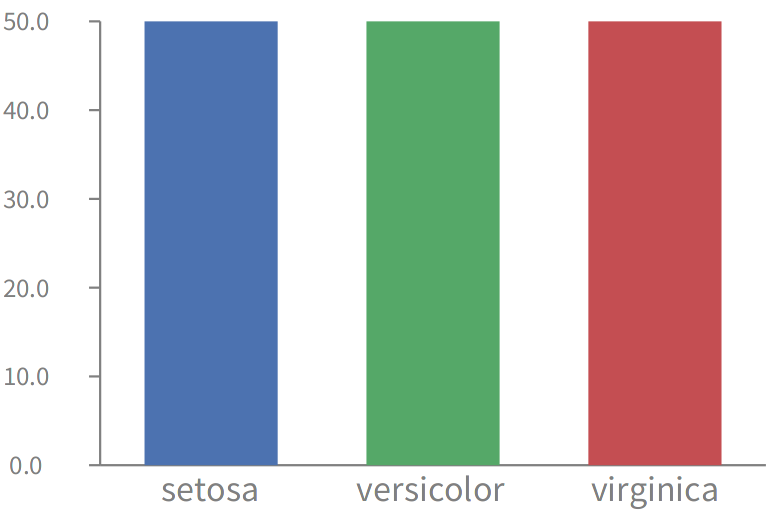
\includegraphics[width=0.75\linewidth]{species_bar}
  \end{center}
\end{figure}

\subsection{Multivariate non-graphical EDA}
\label{sec:multi-non}

Multivariate non-graphical EDA shows the relationship between two variables in form of either cross-tabulation (categorical data) or statistics (quantitative data).

\subsection{Multivariate graphical EDA}
\label{sec:multi-graph}

\begin{figure}[H]
  \begin{center}
  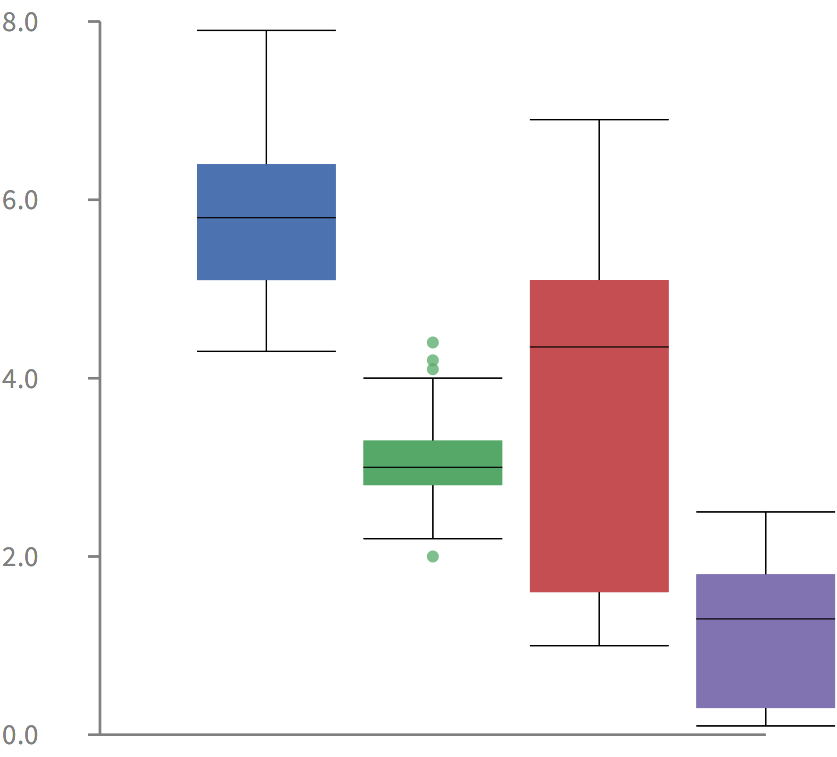
\includegraphics[width=0.75\linewidth]{boxplot}
  \end{center}
\end{figure}

Let's look at the scatterplot of two statistical variables representing the width and length of a sepal. To do that we ask our DataFrame to give us specific columns, in our case, \texttt{sepal\_width} and \texttt{sepal\_length}, then we ask these columns (the result will be another DataFrame) to visualize themselves.

\begin{lstlisting}
vars := data columns: #(sepal_width sepal_length).
vars scatterplot.
\end{lstlisting}

\begin{figure}[H]
  \begin{center}
  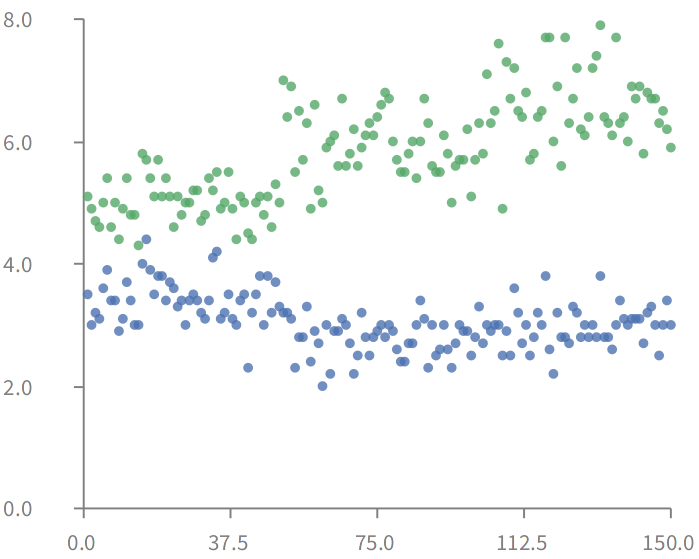
\includegraphics[width=0.75\linewidth]{sepal_wl_scatter}
  \end{center}
\end{figure}

% \section{Discussion}
% \label{sec:discussion}
%
% Discussion of actual solution \emph{vs.} initial constraints from
% \ref{sec:problem}. Explain the space of the solution, why we made it this way.
%
% Evaluation of the solution. How does the solution meet the criteria? Where
% does it succeed or fails...


% \section{Related Works}
% \label{sec:related}
%
% Other solutions in the domain, and a real comparison of our contribution with
% solutions from other people.

\section{Conclusion \& Future work}
\label{sec:conclusion}
At the time of writing this paper DataFrame is capable of...
However, a lot of functionality is still missing. For example, we need tools for
\begin{itemize}
  \item data wrangling
  \item data aggregation and grouping
\end{itemize}

% \section{Conclusion}


% In this paper, we \textsf{looked}\xspace at problem P with this context and these
% constraints. We proposed solution S. It has such good points and such not so
% good ones. Now we could do this or that.


% \section*{macro example}
%
% \ct{look at it this is code }
% \begin{code}{}
% Class>>nknkjbkjbkjb
%     \{| grgr | 
%     grgrgrgg 
%     a := 
% \end{code}

% \subsection*{Acknowledgements} This work was supported by Ministry of Higher Education and Research, Nord-Pas de Calais Regional Council, FEDER through the 'Contrat de
% Projets Etat Region (CPER) 2007-2013',  the Cutter ANR project, ANR-10-BLAN-0219 and the MEALS Marie Curie Actions program FP7-PEOPLE-2011-
% IRSES MEALS (no. 295261). 

% \bibliographystyle{plain}
% \bibliography{foo.bib}

% \appendix
% 
% \section{Lots of Furry Technical Details}

\bibliographystyle{plain}
\bibliography{pharoeda}

%\bibliography{rmod,others}
%\end{multicols}
\end{document}

%%% Local Variables: 
%%% coding: utf-8
%%% mode: latex
%%% TeX-master: "main"
%%% TeX-PDF-mode: t
%%% End:
